\documentclass[handout]{beamer}
\usepackage{amsmath,amssymb,amsthm}
\usepackage[utf8]{inputenc}
\usepackage[russian]{babel}
\usepackage{alltt}
\usepackage{xcolor}
\usepackage{hyperref}
\usepackage{adjustbox}
\usepackage{minted}
\usepackage{graphicx}
\graphicspath{{pictures/}}
\usepackage{caption}

\newlength\someheight
\setlength\someheight{3cm}

\definecolor{urlcolor}{HTML}{9b84ff}
\hypersetup{pdfstartview=FitH,urlcolor=urlcolor, colorlinks=true}

\usetheme{default}
\usecolortheme{default}
\logo{
\includegraphics[width=.1\textwidth]{logo1.png}}

\title{Научно-исследовательская практика}
\subtitle{Nerdle Game на Python}
\author{Климентий Конрат\\\\\ Андрей Белов}
\institute{Институт физико-математических наук и информационных технологий БФУ им. И. Канта}
\date{1 июля 2022 года}

\newtheorem*{myproblem}{Решить задачу}
\newtheorem*{chinesethi}{Китайская теорема об остатках}
\newtheorem*{solve1}{Решение}
\newtheorem*{solve2}{Упрощение процесса решения с помощью кода}
\begin{document}
	
	\section{Титульный лист}
	\begin{frame}
		\titlepage
	\end{frame}
	
	\section{Формулировка задания}
	\begin{frame}
		\frametitle{Формулировка задания}
		\textbf{Задание:}
		\setbeamertemplate{itemize items}[circle]
		\begin{itemize}
            \item Релизация настольной игры \href{https://nerdlegame.org/}{Nerdle} при помощи Python 
        \end{itemize}
        \textbf{Использованные инструменты:}
        \begin{itemize}
            \item Язык \href{https://www.python.org/}{Python 3.10}
            \item Список используемых библиотек: random, re, Calculus.
        \end{itemize}
	\end{frame}
    
    \section{О игре}
    \begin{frame}{О игре}
        \item Nerdle — это игра в жанре головоломки, разработанная Marcus Tettmar. Она была выпущена в 2022. Её издателем выступила компания Marcus Tettmar.
        \item Правила очень просты: вам нужно точно угадать математическое равенство длины k (считая знаки) за n попыток. 
    \end{frame}
    
    \section{Механики игры}
    \begin{frame}{Механики игры}
    Игроку даются символы от 0 до 9 и знаки арифметических операций, среди которых однозначно присутствующим знаком является символ '='.
    В каждой новой попытке игрок вводит свой вариант истинного выражения, чтобы узнать, какие цифры и арифметические знаки входят в уравнение. Если в уравнении вообще нет цифры или знака, то символ помечается путём его дальнейшего не отображения. Если число или знак есть в уравнении, но в неправильном месте, тогда символ останется в отображаемом списке; если в точном месте, соответствующий знак '?' "открывается".   
    \end{frame}
        
    \section{Стратегия}
    \begin{frame}{Стратегия}
         \item В Nerdle каждая из наших догадок должна заполнить 8 пустых серых плиток. В распоряжении игрока набор цифр (0, 1, 2, 3, 4, 5, 6, 7, 8, 9), набор операторов (+, -, *, /), и символ '='. В отличие от угадывания слов, решение числового уравнения сразу; может быть более сложным.
         \item Существует две основные стратегии. 
         \item Первая стратегия заключается в том чтобы как можно использовать уникальных цифр в первых двух попытках
         \item Вторая стратегия заключается в том чтобы использовать как можно больше операторов в первых двух попытках
    \end{frame}
    
    \section{Лучшие числа для старта}
    \begin{frame}{Лучшие числа для старта}
        \item Числовое уравнение с первым предположением, которое помогает быстрее фильтровать цифры 
           48 - 36 = 12
        \item 8 из 10 чисел, введенных непосредственно в игру, дают вам преимущество в получении информативной обратной связи. Это может значительно сократить общее количество попыток, которые  придется использовать, если вы вслед за первой попыткой составите уравнение, которое включает в себя благоприятную комбинацию оставшихся неиспользуемых чисел (5, 7, 9, 0) и операторов (+, /, *), например, 9 * 8 - 7 = 65 или 47 - 5 * 9 = 2.
    \end{frame}
    
    \section{Лучшие числа для старта}
    \begin{frame}{Лучшие числа для старта}
        \item Лучшие первые уравнения для старта: \\9 * 8 - 7 = 65 \\0 + 12 / 3 = 4 \\47 - 5 * 9 = 2 \\12 / 4 + 0 = 3 \\17 - 3 * 4 = 5 \\56 / 8 + 2 = 9
    \end{frame}
    
    \section{Примеры хороших уравнений для победы}
     \begin{frame}{Примеры хороших уравнений для победы}
     
        \item Когда все символы в уравнениях уникальны, они дают вам информацию о существовании 7 из 14 чисел и операторов. По этой логике лучшими уравнениями для первых двух догадок являются:\\9 * 8 - 7 = 65 \\0 + 12 / 3 = 4
        \item Похожие но не настолько эффективные уравнения 17 - 3 * 4 = 5 \\56 / 8 + 2 = 9
        Стоит использовать уравнения с ответом 0, например: 12 / 3 - 4= 0, в таком случае исключаются все операции с одиноким 0.
        \item Для победы не стоит использовать уравнения с начальными нулями такие как 12 + 03 = 15
        а так же отрицательные числа -35 + 2 = -33, несколько операторов единовременно 1 +* 2
    \end{frame}

    \section{Код}
    \begin{frame}{Список используемых библиотек}
        \centering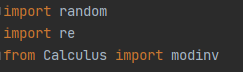
\includegraphics[width=4in, keepaspectratio]{Библиотеки.png}
    \end{frame}
    \section{}
    
    \section{Код}
    \begin{frame}{Модуль Calculus}      
        \centering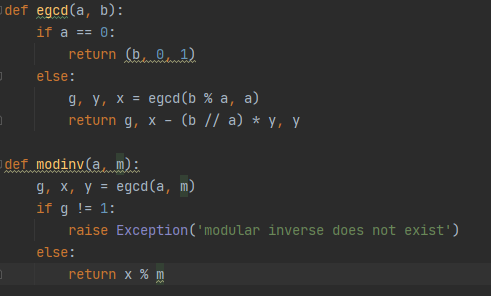
\includegraphics[width=4in, keepaspectratio]{Calculus.png}
    \end{frame}
    
    \section{Код}
    \begin{frame}{Класс определения операции}
        \centering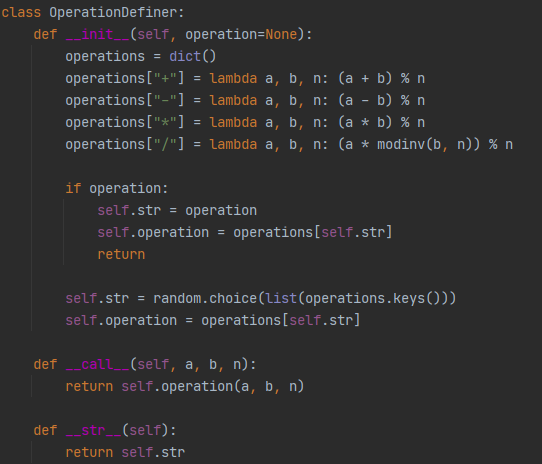
\includegraphics[width=3in, keepaspectratio]{OperationDefiner.png}
    \end{frame}
    \section{}
    

    \section{Код}
    \begin{frame}{Класс игрового движка и его конструктор}
        \centering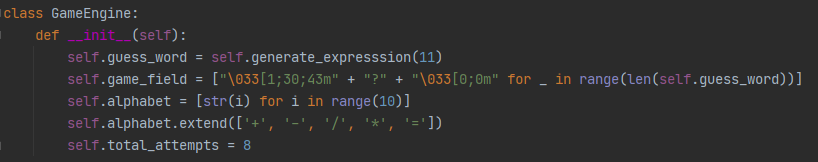
\includegraphics[width=4in, keepaspectratio]{GE - Конструктор.png}
    \end{frame}

    \section{Код}
    \begin{frame}{Метод генерации выражения для игровой ситуации}
        \centering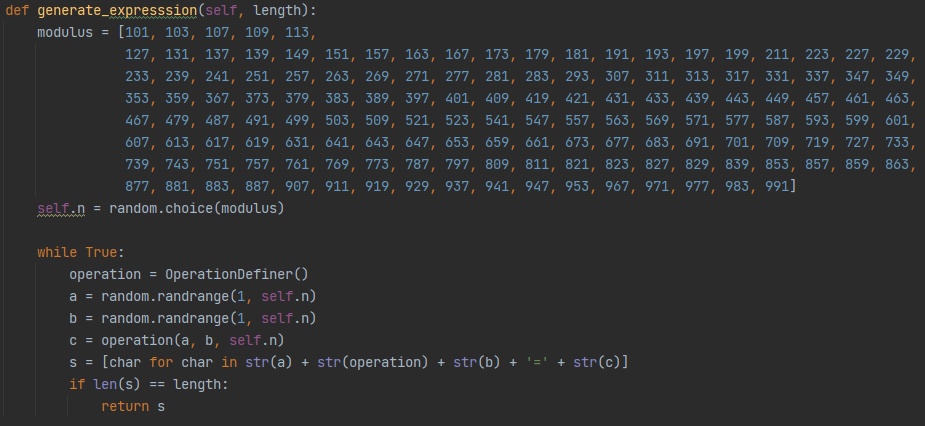
\includegraphics[width=4in, keepaspectratio]{GE - Генерация выражения.png}
    \end{frame}

    \section{Код}
    \begin{frame}{Метод отображения игровой доски в терминале с "подсветкой"}
        \centering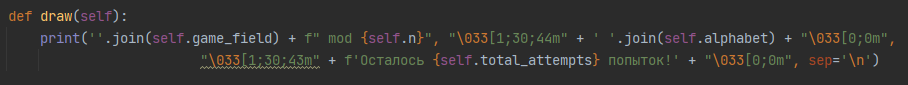
\includegraphics[width=4in, keepaspectratio]{GE - Отображение.png}
    \end{frame}

    \section{Код}
    \begin{frame}{Метод обновления игровых данных}
        \centering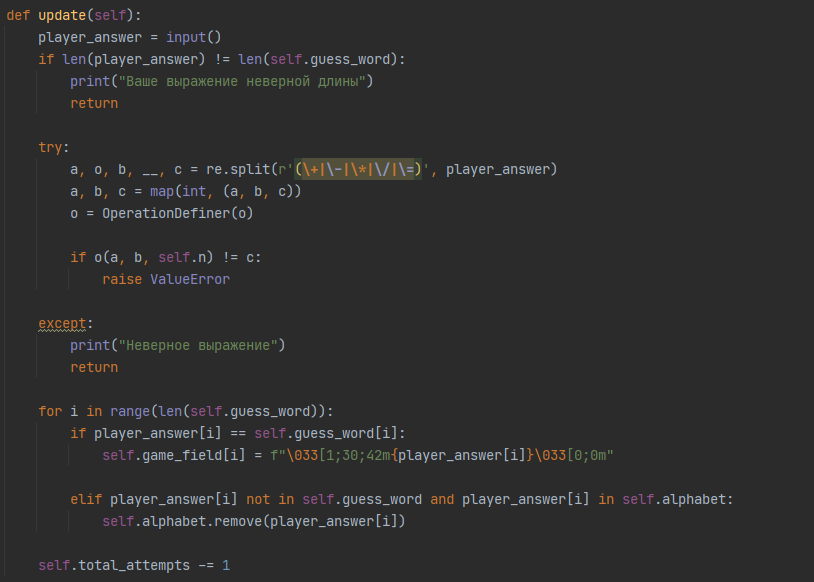
\includegraphics[width=4in, keepaspectratio]{GE - Обновление.png}
    \end{frame}

    \section{Код}
    \begin{frame}{Метод проверки победы игрока}
        \centering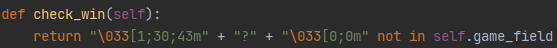
\includegraphics[width=4in, keepaspectratio]{GE - Проверка победы.png}
    \end{frame}

    \section{Код}
    \begin{frame}{Старт игры и игровой цикл}     
        \centering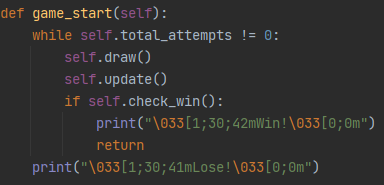
\includegraphics[width=4in, keepaspectratio]{GE - Игровой цикл.png}
    \end{frame}
\end{document}